\documentclass[notes,compress,serif,professionalfont]{beamer}
\usetheme{boxes} %Boadilla, Berkeley, Dresden, Rochester, Pittsburgh
\useoutertheme{miniframes} %split, shadow, infolines, default
\usepackage{hyperref}
\usepackage{pxfonts}
\usepackage{amsmath}
\usepackage{amssymb}
\usepackage{amsfonts}
\usepackage{enumerate}
\usepackage{xcolor}
\usepackage{multirow}
\usepackage{tikz}
\usepackage{subfigure}
\usetikzlibrary{arrows,shapes}
\beamertemplateballitem % make bullets and items fancy balls
\useheadtemplate{%
\vbox{%
\vskip1pt%
\beamerline{\insertnavigation{\paperwidth}}%
\vskip-5pt
}
}
%\renewcommand{\frametitle}[1]{\begin{center}\textbf{#1}\end{center}}

\begin{document}
\title{Title}
\author{Harry J.~Paarsch}
\date{xx June 2024}

\begin{frame}
  \titlepage
\end{frame}

\section{Introduction}

\begin{frame}
\frametitle{Motivation}
\begin{itemize}

\item<+-> The quick brown fox jumped over the lazy dogs.

\item<+-> The quick brown fox jumped over the lazy dogs.
% \item The quick brown fox jumped over the lazy dogs.

% \item The quick brown fox jumped over the lazy dogs.

       \begin{itemize}
             \item A
	     \item B
	     \item C
       \end{itemize}

\end{itemize}
\end{frame}

\begin{frame}\frametitle{The Price of \emph{Lamotrigene}}
\begin{center}
    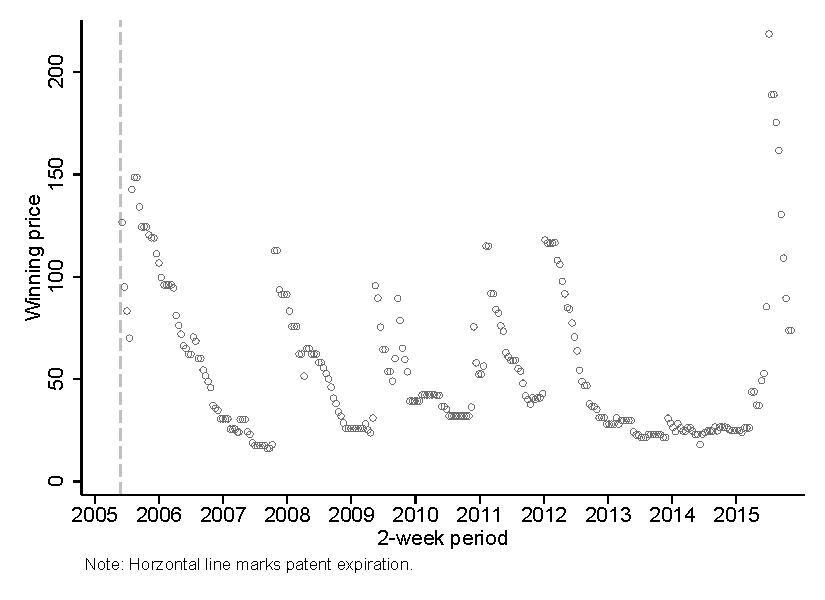
\includegraphics[width=.8\textwidth]{Sample-Figure.pdf}
\end{center}
\end{frame}




In this appendix, I present an exerpt of the rewards credit cards dataset, and describe in more detail how the static benefits were handled. 
I also present tables of the spending budgets and income levels that were used for the sensitivity analysis and Monte Carlo simulation. 

Figure~\ref{fig:CreditCardsCSV} shows an exerpt of the credit cards dataset. 
Note the that columns ``id'' contains duplicate numbers for:
\begin{itemize}
    \item cards that are mutually exclusive (Chase Sapphire Preferred and Reserve);
    \item cards that have custom reward categories, but the user can only hold one of these cards at a time (Citi Custom Cash);
    \item cards that have identical rewards, but are from different banks (Citi Custom Cash and Wells Fargo Active Cash).
\end{itemize}
Having identical ``id'' numbers for these cards makes it easier to deal with these situations in the algorithm, after one of these cards is selected for the portfolio (namely by setting all values to zero of cards with the same ``id'').

If a card has a travel or food credit, this credit was taken as a benefit at full value (column ``benefit\_credits''). Benefits that are not easily combined between different credit cards, such as a ``Global Entry / TSA Precheck'' credit, airport lounge access, and CLEAR membership credit, received a ``1'' flag in the columns ``benefit\_globalentry,'' ``benefit\_lounge,'' and ``benefit\_clear,'' respectively (or ``0'' if not available). 
This allows for an easy solution in the code to avoid counting these benefits multiple times, when in practice they can only be used once. 
The \$100 ``Global Entry / TSA Precheck'' credit every five years is assumed as a \$20 yearly benefit. Airport lounge access is valued at \$40, which is approximately the value of two free meals with drinks. 
The CLEAR membership credit is a \$189 value. 
Once a card is added to the portfolio in the recommendation algorithm, all these values are multiplied by $1-$ the flag of the selected card, which means the benefit is ``turned off'' after its first use. 

A boolean column ``cash\_only'' was added to indicate if the card is cashback only (TRUE), or if the card allows for higher-valued travel redemptions (FALSE).
This could potentially be used to filter for certain user preferences.
The columns ``base\_value'' and ``travel\_value'' were populated with the point valuations from \citet{nerdwallet:2024}, which are also shown in Table~\ref{tab:PointValues}.
The final 36 columns (two for each spending category) contain the point multipliers and their limits (``\ldots\_cap''), sourced from the website \url{https://www.allcards.com}, as well as from the bank's websites. 
All these credit card data were manually recorded in a Google Sheet, and finally saved to the file \texttt{CreditCards.csv}. 

\begin{landscape}
    \begin{figure}[t!h]
        \begin{center}
        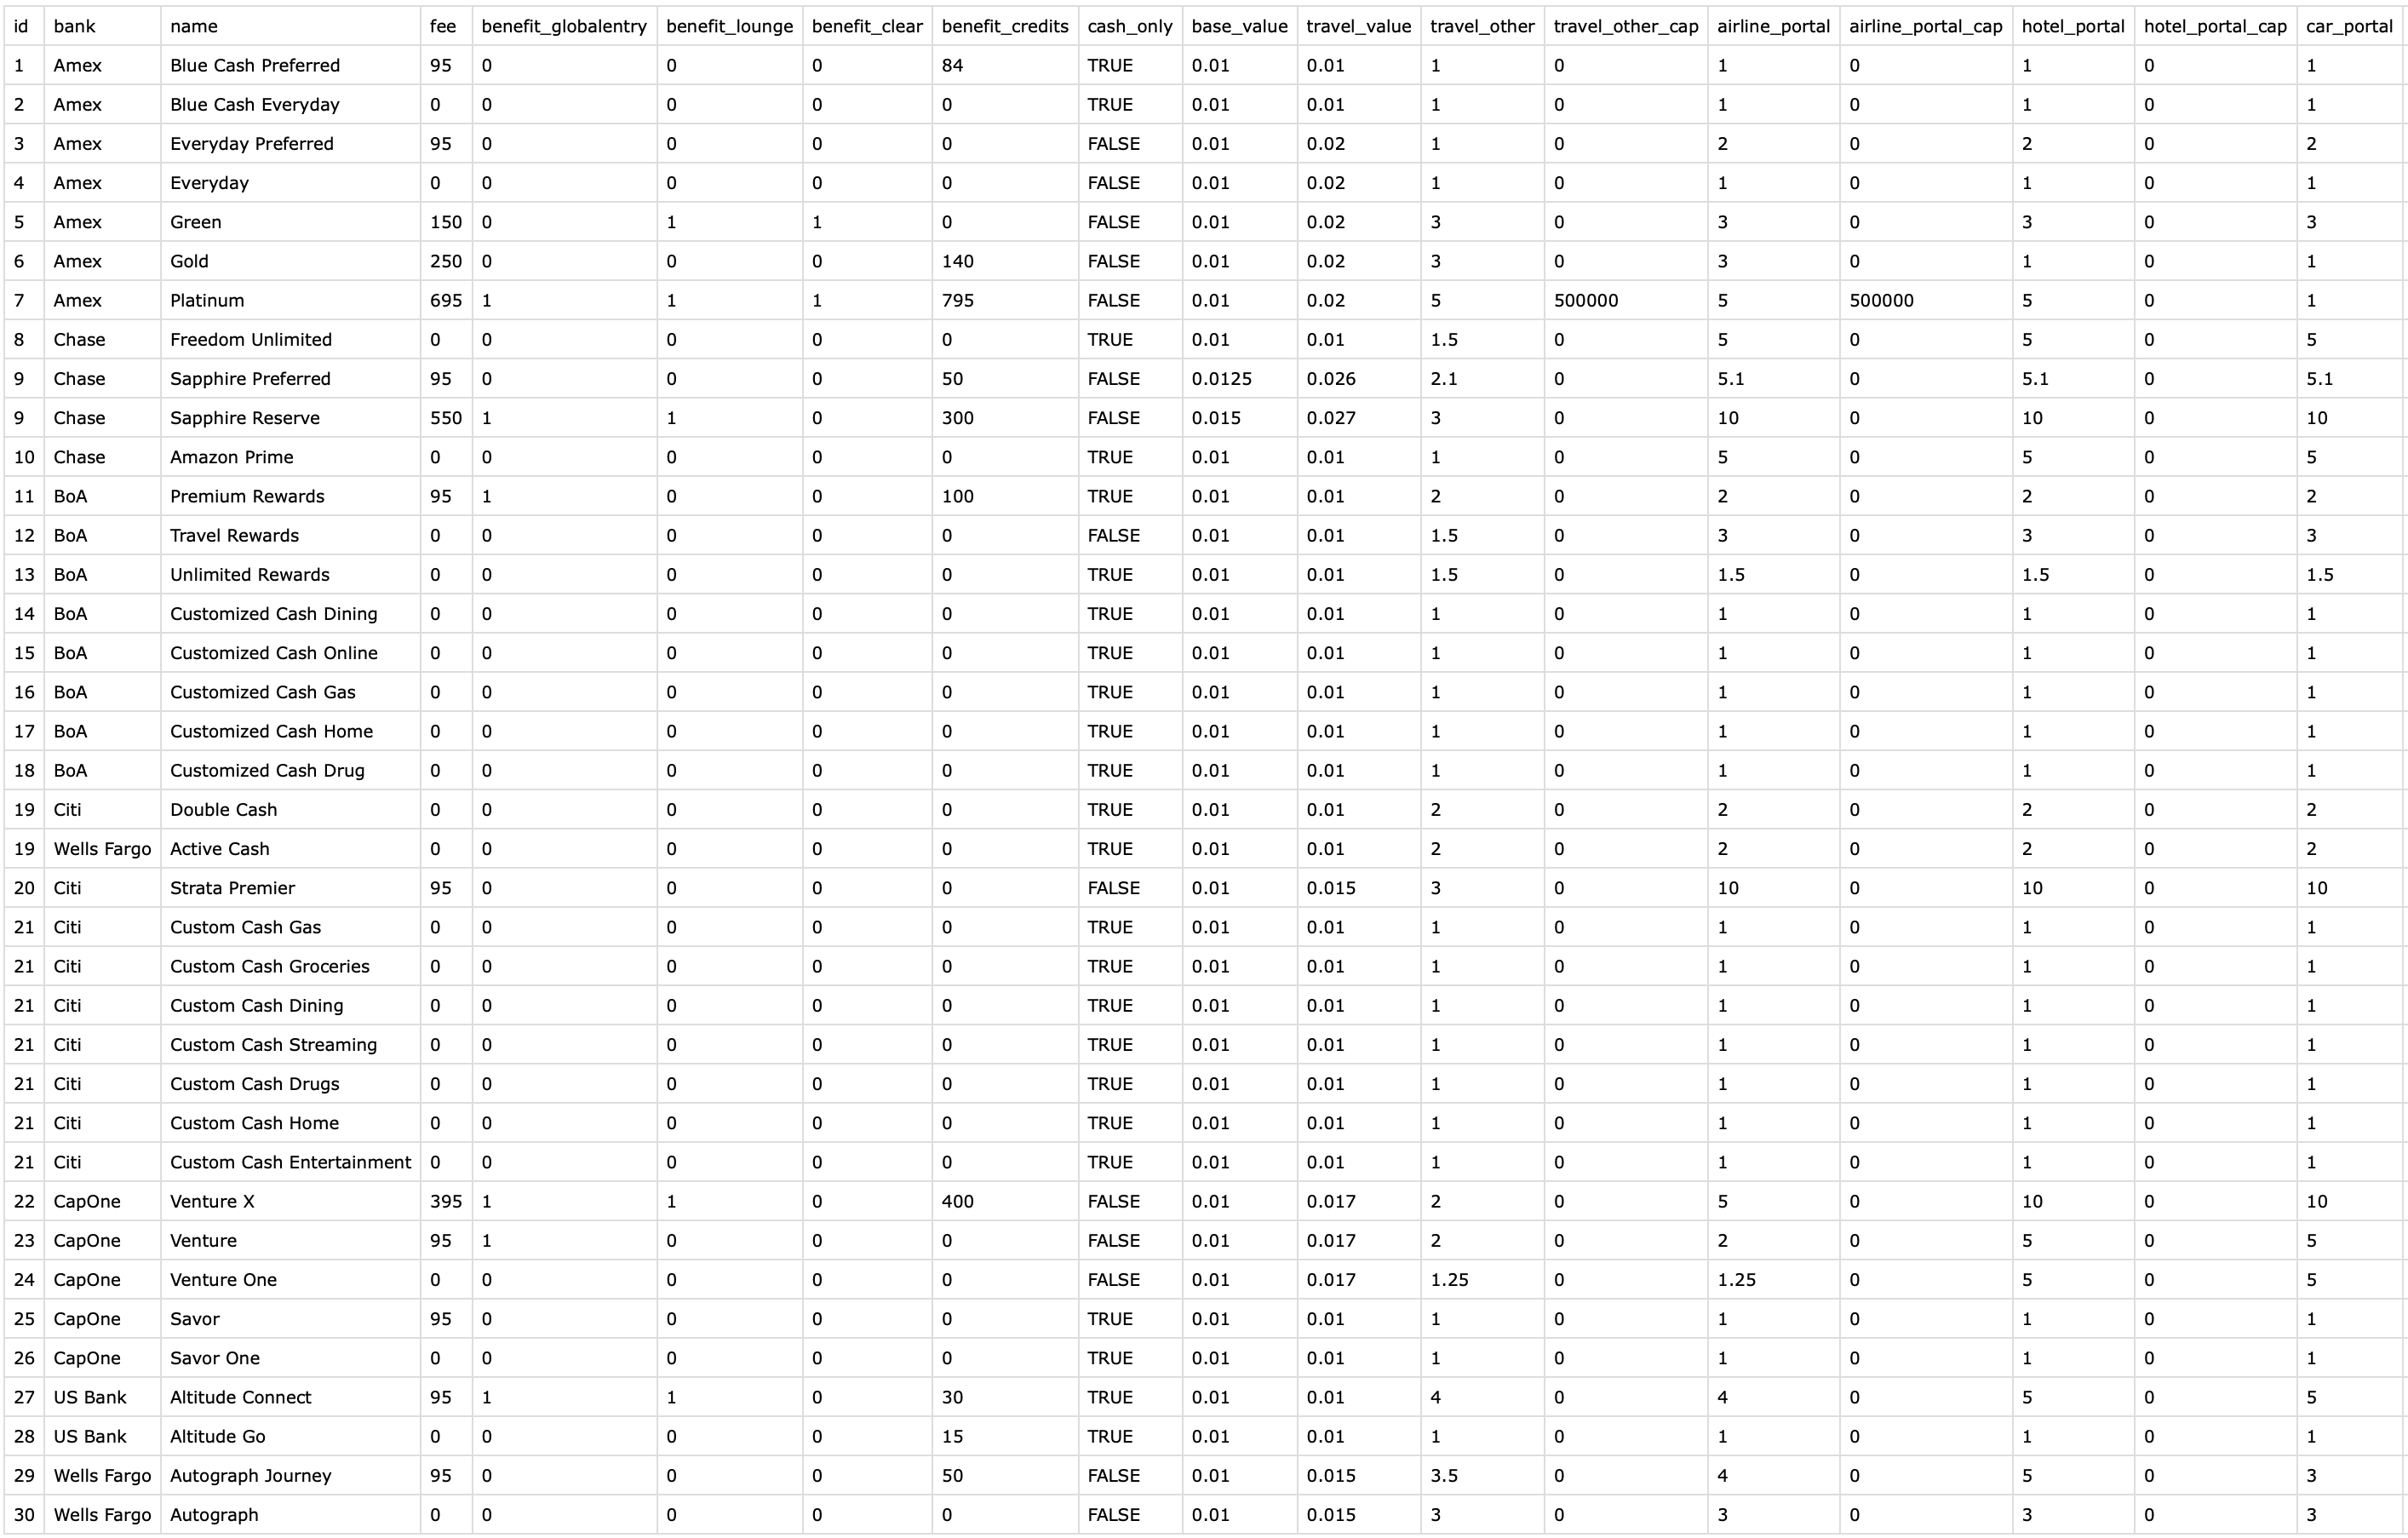
\includegraphics[scale=0.45]{../Misc/CreditCardsCSV.png}
        \caption{Exerpt of the file \texttt{CreditCards.csv} with all the 38 credit cards shown, but only 4 of the 18 spending categories with multipliers and their corresponding caps.}
        \label{fig:CreditCardsCSV}
        \end{center}
    \end{figure}
\end{landscape}

% Table with Point Values, based on NerdWallet: https://www.nerdwallet.com/article/travel/airline-miles-and-hotel-points-valuations 
\begin{table}[t!bh]
    \centering
    \begin{tabular}{ r c c} 
        \hline
         & Base Value $v_{b}$ [\$] & Travel Value $v_{t}$ [\$] \\ 
        \hline
        Amex Cashback Cards & 0.01 & 0.01 \\
        Amex Membership Rewards Cards & 0.01 & 0.02 \\
        Chase Cashback Cards & 0.01 & 0.01 \\
        Chase Sapphire Preferred & 0.0125 & 0.026 \\
        Chase Sapphire Reserve & 0.015 & 0.027 \\
        Bank of America (all cards) & 0.01 & 0.01 \\
        Citi Strata Premier & 0.01 & 0.015 \\
        Citi Cashback Cards & 0.01 & 0.01 \\
        Capital One Miles (Venture Cards) & 0.01 & 0.017 \\
        Capital One Cashback (Savor Cards) & 0.01 & 0.01 \\
        US Bank (all cards) & 0.01 & 0.015 \\
        Wells Fargo (all cards) & 0.01 & 0.015 \\
        \hline
    \end{tabular}
    \caption{Base and travel point values for various types of rewards credit cards. Note the elevated base values for the Chase Sapphire travel cards, which assumes redeeming the points in Chase's travel portal. Source: \citet{nerdwallet:2024}.}
    \label{tab:PointValues}
\end{table}



Table~\ref{tab:BudgetExtended} shows how the mapping between credit card categories and the items from the CES was performed, for the average consumer in 2022 with an income (before taxes) of \$94,003.
Finally, Table~\ref{tab:BudgetIncome} shows the credit card spending budgets (as percentages of gross income), separated by income level. 

\begin{landscape}
    % Table of average Credit Card Budget from the 2022 BLS Consumer Expenditure Survey    
    \begin{table}[t!bh]
    \centering
    \begin{tabular}{ r c c l} 
        \hline
        Category & Expenditure [\$] & \% & Consumer Expenditure Survey Items \\ 
        \hline
        Everything else	& 7,786 & 20.18 & Household operations, Vehicle finance charges, Maintenance and repairs, \\
        & & & Vehicle insurance, Medical services and supplies, Reading, Tobacco, Miscellaneous \\
        Groceries & 6,362 & 16.49 & Food at home, Laundry and cleaning supplies, Other household products \\
        Dining & 4,222 & 10.94 & Food away from home, Alcoholic beverages \\
        Gas	& 3,120	& 8.09 & Gasoline, other fuels, and motor oil \\
        Utility	& 3,117	& 8.08 & Utilities, fuels and public services\\
        Home improvement & 2,606 & 6.76 & Household furnishings and equipment \\
        Online shopping	& 1,881	& 4.87 & 50\% Apparel and services, Pets, toys, hobbies, and playground equipment\\
        Drug store	& 1,481 & 3.84 & Drugs, Personal care products and services \\
        Travel (other) & 1,460 & 3.78 & 50\% Other lodging, 50\% Vehicle rental, leases, licenses and other charges, \\
        & & & 50\% Public and other transportation \\
        Phone & 1,431 & 3.71 & Telephone services\\
        Streaming & 1,020 & 2.64 & Audio and visual equipment and services\\
        Department store & 973 & 2.52 & 50\% Apparel and services \\
        Entertainment & 833 & 2.16 & Fees and admissions \\
        Cable internet & 698 & 1.81 & Other entertainment supplies, equipment, and services \\
        Hotel (portal) & 644 & 1.67 & 50\% Other lodging \\
        Airline (portal) & 423 & 1.10 & 50\% Public and other transportation\\
        Car rental (portal) & 394 & 1.02 & 50\% Vehicle rental, leases, licenses and other charges \\
        Office supplies & 128 &	0.33 & Postage and stationery \\
        \hline
        \hline
        Total & 38,576	& 100.00 & \\
    \end{tabular}
    \caption{The average credit card budget as derived from the 2022 BLS Consumer Expenditure Survey. The corresponding mean income (before taxes) is \$94,003, showing that, with this budget, 41 percent of the gross income can be spend on credit cards. The first column lists the 18 credit card categories that are used throughout this project, while the last column shows how the expenditure items were mapped to each of the credit card categories.}
    \label{tab:BudgetExtended}
\end{table}


    % Table of average Credit Card Budgets from the 2022 BLS Consumer Expenditure Survey, separated by income bins
    \begin{table}[t!bh]
    \centering
    \begin{tabular}{ r c c c c c c c c c c} 
        \hline
          & \multicolumn{10}{c}{Expenditures as percentage of gross income} \\ 
         \hline
          & All & Less & \$15,000  & \$30,000 & \$40,000  & \$50,000  & \$70,000 & \$100,000  & \$150,000 & \$200,000 \\
          & consumer  &  than  & to  & to  & to & to & to & to & to &  and  \\
          & units & \$15,000 & \$29,999 & \$39,999 & \$49,999 & \$69,999 & \$99,999 & \$149,999 & \$199,999 &  more \\
        \hline
        Everything else	& 8.28 & 46.26 & 16.61 & 15.49 & 12.55 & 11.05 & 9.66 &	7.92 & 6.50 & 4.86 \\
        Groceries & 6.77 &	55.85 &	17.33 &	13.17 &	11.73 &	9.89 &	7.97 &	6.31 &	5.23 &	3.16 \\
        Dining &  4.49 &	22.10 &	8.02 &	6.52 &	6.42 &	5.65 &	4.57 &	4.58 &	4.15 &	3.09 \\
        Gas	&  3.32 &	19.86 &	7.71 &	6.61 &	5.66 &	5.17 &	4.20 &	3.37 &	2.62 &	1.46 \\
        Utility	& 3.32 &	24.30 &	10.08 &	7.72 &	6.25 &	4.96 &	3.79 &	2.94 &	2.37 &	1.50 \\
        Home improvement & 2.77 &	12.41 &	5.16 &	5.07 &	3.74 &	3.27 &	2.90 &	2.64 &	2.65 &	1.96 \\
        Online shopping	& 2.00 &	5.61 &	3.89 &	3.11 &	2.96 &	2.56 &	2.42 &	1.85 &	1.75 &	1.24 \\
        Drug store	& 1.58 &	7.92 &	3.95 &	2.88 &	2.63 &	1.32 &	1.84 &	1.35 &	1.24 &	0.80 \\
        Travel (other) & 1.55 &	3.27 &	2.01 &	2.09 &	1.65 &	1.55 &	1.30 &	1.40 &	1.41 &	1.57 \\
        Phone & 1.52 &	9.85 &	4.14 &	3.20 &	2.88 &	2.29 &	1.85 &	1.51 &	1.19 &	0.62 \\
        Streaming & 1.09 &	6.81 &	2.98 &	2.37 &	1.84 &	1.43 &	1.29 &	1.06 &	0.85 &	0.53 \\
        Department store & 1.03 &	0.00 &	1.77 &	1.29 &	1.62 &	1.29 &	1.24 &	1.00 &	0.84 &	0.68 \\
        Entertainment &  0.89 &	1.90 &	0.65 &	0.82 &	0.69 &	0.84 &	0.79 &	0.80 &	1.10 &	0.91 \\
        Cable internet & 0.74 &	0.94 &	0.47 &	0.00 &	0.33 &	0.00 &	0.00 &	0.52 &	0.00 &	0.74 \\
        Hotel (portal) & 0.68 &	0.00 &	0.72 &	0.81 &	0.63 &	0.60 &	0.52 &	0.58 &	0.60 &	0.79 \\
        Airline (portal) & 0.45 &	1.90 &	0.61 &	0.64 &	0.50 &	0.44 &	0.37 &	0.40 &	0.39 &	0.46 \\
        Car rental (portal) & 0.42 &	1.38 &	0.68 &	0.64 &	0.52 &	0.52 &	0.41 &	0.43 &	0.42 &	0.32 \\
        Office supplies &  0.14 &	1.15 &	0.00 &	0.26 &	0.24 &	0.21 &	0.15 &	0.12 &	0.11 &	0.06 \\
        \hline
        \hline
        Total & 41.04 &	221.52 & 86.78 & 72.68 & 62.85 & 53.02 & 45.28 & 38.78 & 33.42 & 24.77 \\
    \end{tabular}
    \caption{The average credit card budget for different income bins, as derived from the 2022 BLS Consumer Expenditure Survey. Note that consumers with an income less than \$15,000 spend more than 200 percent of their income, which is likely explained by receiving gifts or loans. This income bin will therefore be ignored in the analysis.}
    \label{tab:BudgetIncome}
\end{table}


\end{landscape}

\end{document}
